\begin{figure}[htbp]\centering
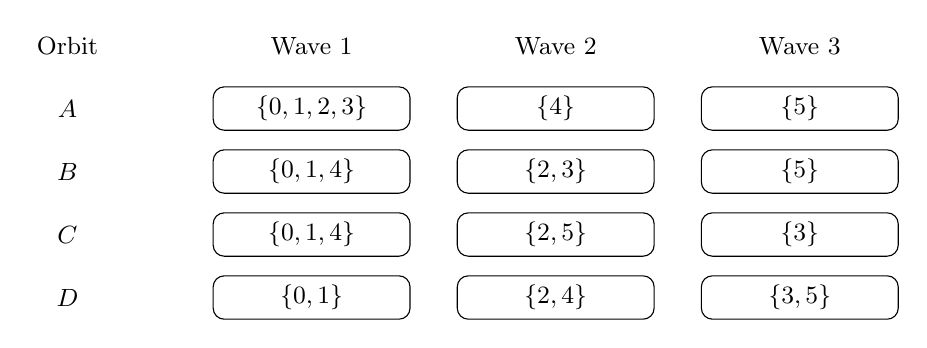
\begin{tikzpicture}[x=3.1cm,y=.8cm,every node/.style={font=\small},
 wave/.style={draw,rounded corners,minimum width=2.5cm,minimum height=.55cm}]
\node at (0,1) {Orbit}; \node at (1,1) {Wave 1};
\node at (2,1) {Wave 2}; \node at (3,1) {Wave 3};
\foreach \y/\lab/\one/\two/\three in {
0/A/{0,1,2,3}/{4}/{5},
-1/B/{0,1,4}/{2,3}/{5},
-2/C/{0,1,4}/{2,5}/{3},
-3/D/{0,1}/{2,4}/{3,5}}{
 \node at (0,\y) {$\lab$};
 \node[wave] at (1,\y) {$\{\one\}$};
 \node[wave] at (2,\y) {$\{\two\}$};
 \node[wave] at (3,\y) {$\{\three\}$};}
\end{tikzpicture}
\caption{Representative six-check partitions in Theorem 3. Here
$G=\{0,1,2,3\}$ and $O=\{4,5\}$. Each orbit is uniform over all
renamings within $G,O$; wave order is uniformly permuted.
$P=7A/8+B/8$ and $Q=9A/10+C/20+D/20$ share the stated pairwise
completion laws. These are complete epochs, unlike the main article's
persistent partial-refresh construction.}
\label{fig:s-wave-partitions}
\end{figure}
